%! Author = Len Washington III
%! Date = 9/8/25

% Preamble
\documentclass[
	lecture={3},
	title={Interior of the Earth}
]{enve201notes}

% Packages

% Document
\begin{document}

\setcounter{chapter}{2}
%<*Lecture-3>
\chapter{Interior of the Earth}\label{ch:interior-of-the-earth}
\section{Quick Facts About Earth}\label{sec:quick-facts-about-earth}
\begin{itemize}
	\item The third planet from the Sun and the fifth-largest planet.
	\item The only place we know of inhabited by living things.
	\item Length of days: 23.9 hours
	\item Length of year: 365.25 days
	\item Distance from Sun: 93,327,712 miles (150,196,428 km)
	\item The name Earth is at least 1,000 years old.
	It was taken from Old English and Germanic.
	Imply it means ``the ground''.
\end{itemize}

\section{The Earth System}\label{sec:the-earth-system}
\begin{itemize}
	\item Only the Earth currently has liquid water among the Solar System's planets.
	\item The Earth lies \win\ the \emph{habitable zone} -- the distance from the Sun at which temperatures range between the boiling and freezing points of water.
	\begin{itemize}
		\item On planets closer to the Sun than the habitable zone, all water evaporates.
		\item On planets farther away, all water exists only as solid ice.
	\end{itemize}
	\item Earth has the potential for life!
\end{itemize}

\section{The Size of Earth}\label{sec:the-size-of-earth}
\begin{itemize}
	\item Eratosthenes observed that if the Earth were spherical, the Sun's rays could not strike two distant locations at the same angle at the same time.
	\begin{itemize}
		\item At noon in Syene (modern Aswan), the Sun was directly overhead and cast no shadow.
		\item At the same time in Alexandria, about 5,000 stadia ($\approx800$ km) to the North, a vertical tower cast a shadow.
		\item Eratosthenes measured the angle between the two and the Sun's rays to be 7.2\textdegree.
		\item Since 7.2\textdegree\ is $\frac{1}{50}$ of a full circle, he concluded that the Earth's circumference must be 50 times the distance between the two cities and it is 250,000 stadia ($\approx39,300$ km).
	\end{itemize}
	\item \emph{Very close to the modern accepted value (40,075.017 km)!}
\end{itemize}

\section{Earth's Rotation}\label{sec:earth's-rotation}
\begin{itemize}
	\item Earth completes one rotation every \emph{23.9 hours} and it takes \emph{365.25 days} to complete one trip around the sun!
	\item Foucault proved that the Earth spins on its axis
\end{itemize}

\subsection{Foucault's Pendulum Experiment}\label{subsec:foucault's-pendulum-experiment}
\begin{figure}[H]
	\centering
	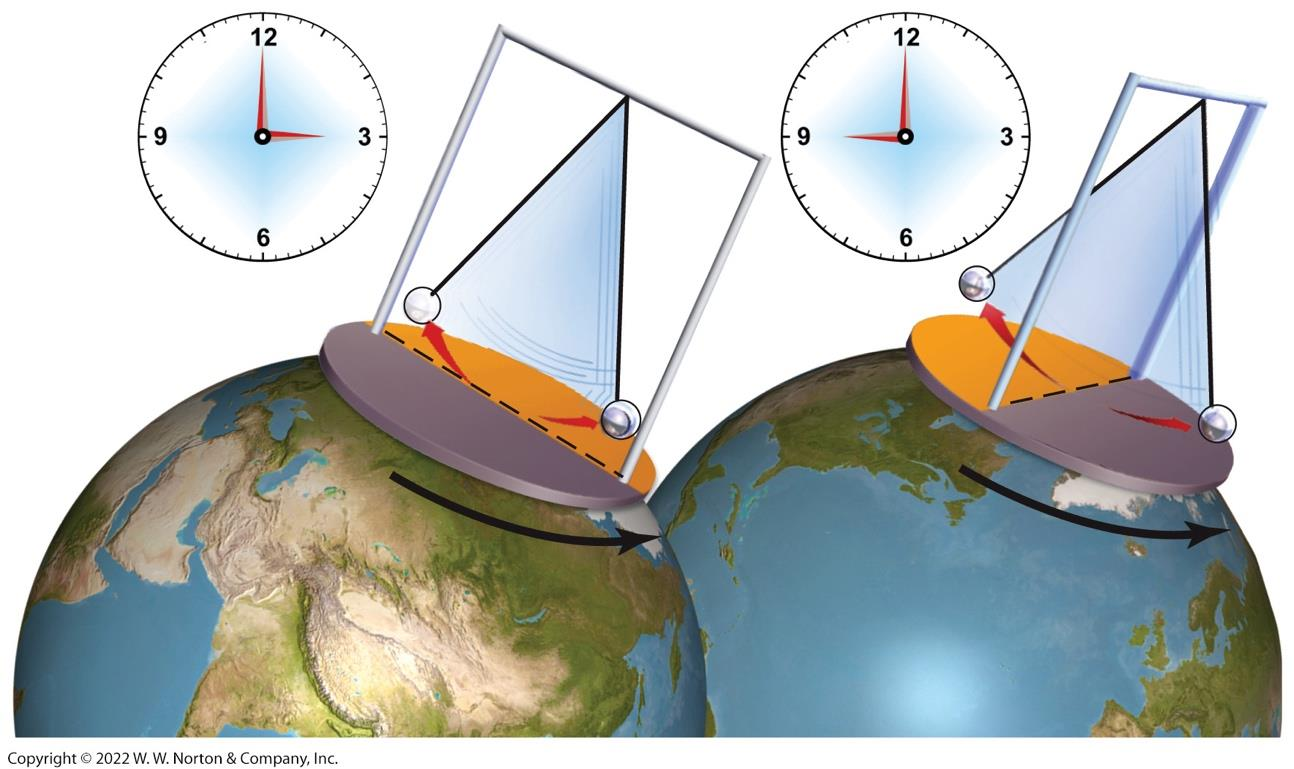
\includegraphics[width=\textwidth]{images/3_foucault_pendulum}
	\caption{Foucault's Pendulum Experiment}
	\label{fig:foucaults-pendulum-experiment}
\end{figure}

\begin{itemize}
	\item At Time 1 (left), the plane in which the pendulum swings is the same as the plane of its frame.
	\item At Time 2 (right), 6 hours later, the plan in which the pendulum swings is perpendicular to the plane of its frame.
\end{itemize}

\subsection{Earth's Axis of Rotation}\label{subsec:earth's-axis-of-rotation}
\begin{itemize}
	\item Earth's axis of rotation is tilted 23.5\textdegree\ \wrt\ the plane of Earth's orbit around the Sun.
	\begin{itemize}
		\item This tilt causes our yearly cycle of seasons.
	\end{itemize}
\end{itemize}

\section{Earth's Structure}\label{sec:earth's-structure}
\begin{itemize}
	\item By the end of the $19^{\text{th}}$ century, researchers realized that the Earth resembles a hard-boiled egg in that it had three principal layers.
	\begin{enumerate}
		\item A not-so-dense crust (like an eggshell),
		\item A thicker and denser solid mantle in the middle (like an egg white),
		\item A very dense core (yolk).
	\end{enumerate}
	\item Earthquake (seismic) waves allowed geologists to refine the model of Earth's interior.
	\item Earth is composed of four main layers:
	\begin{itemize}
		\item Inner core
		\item Outer core
		\item Mantle
		\item Crust
	\end{itemize}
\end{itemize}

\subsection{Earth's Crust}\label{subsec:earth's-crust}
\begin{itemize}
	\item Outermost layer of the Earth
	\item Two types of crust:
	\begin{itemize}
		\item Oceanic crust underlies the seafloor and is thinner (7-10 km) and denser.
		\item Continental crust underlies continent and is thicker (25-70 km) and less dense.
	\end{itemize}
	\item Earth's crust is comprised of, mostly, eight different elements.
	Of these, oxygen and silicon account for 74.3\% by weight.
\end{itemize}

\subsection{Earth's Mantle}\label{subsec:earth's-mantle}
\begin{itemize}
	\item 2,820- to 2,890-km thick shell that surrounds the core.
	\item The mantle can be divided into two sublayers: upper mantle and lower mantle.
	\item Almost all of the mantle is solid rock, but the mantle at a great depth stays so hot that it is enough to flow (at a rate of less than 15 cm/year).
	\item The temperature of the mantle vary \w\ location:
	\begin{itemize}
		\item Warmer regions of mantle are less dense than adjacent cooler regions.
		\item Warmer regions tend to flow upward, while cooler regions flow downward.
		\item \emph{The mantle undergoes very flow convection!}
	\end{itemize}
\end{itemize}

\subsection{Earth's Core}\label{subsec:earth's-core}
\begin{itemize}
	\item The core is the densest layer - consists of iron alloy ($>80\%$ iron mixed \w\ nickel and lesser amounts of sulfur, oxygen, silicon, and other elements).
	\item Core is divided into two parts:
	\begin{itemize}
		\item Outer core (2,890-5,155 km) consists of liquid iron alloy.
		\item Inner core (5,155-6,371 (the center) km) consists of solid iron alloy.
		\item Even though the inner core is hotter than the outer core, the inner core stays solid \bc\ it endures immense pressure.
	\end{itemize}
	\item The iron alloy of the outer core can flow, and this flow generates the Earth's magnetic field.
\end{itemize}

\subsection{Pressure and Temperature Inside the Earth}\label{subsec:pressure-and-temperature-inside-the-earth}
\begin{itemize}
	\item Pressure increases \w\ depth, and at the Earth's center, it is estimated to reach about 3,600,000 atm.
	\item Temperature also increases \w\ depth, approaching 6,000\textdegree{}C at the core.
	\item The rate of temperature increase \w\ depth is called the \textit{geothermal gradient}.
	\begin{itemize}
		\item 15-30\textdegree{}C/km in the upper part of crust.
		\item At greater depth, less than 10\textdegree{}C/km.
	\end{itemize}
\end{itemize}

\section{Earth's Surface}\label{sec:earths-surface}
\begin{itemize}
	\item Dry land covers 30\% of the surface.
	\item Water covers the remaining 70\% of the surface, but most surface water contains salt and resides in the oceans.
	\item \emph{Topography} shows variation in elevation on both the land surface and beneath the ocean.
	\item A \emph{hypsometric curve} indicate the proportion of Earth's solid surface at different elevations.
	\begin{itemize}
		\item Earth's surface is mostly continent (plains and shelf) or ocean floor.
		\item Mountains and deep-sea trenches cover relatively little area.
		\item Change in sea level would dramatically change the area of dry land.
	\end{itemize}
\end{itemize}

\section{Earth's Atmosphere}\label{sec:earth's-atmosphere}
\begin{itemize}
	\item The Earth is wrapped in a gaseous cloak called the atmosphere.
	\item This atmosphere is made of a mixture of gases that we call air.
	\begin{itemize}
		\item Nitrogen (78\%) and oxygen (21\%) are the dominant.
		\item Other gases include argon, carbon dioxide, neon, methane, ozone, carbon monoxide, and sulfur dioxide.
		\item Air also contains variable amounts of water vapor at lower elevation.
	\end{itemize}
	\item Other terrestrial planets have atmosphere, but mostly \ce{CO2} gas.
	\item The density of the atmosphere increases closer to the Earth's surface, and atmospheric pressure decreases \w\ elevation.
	\item However, temperature does not follow a simple decrease--it varies by layer.
	\begin{itemize}
		\item Troposphere
		\item Stratosphere
		\item Mesosphere
		\item Thermosphere
	\end{itemize}
	\item All weather occurs in the \emph{Troposphere}.
\end{itemize}

\section{Earth Materials}\label{sec:earth-materials}
\begin{itemize}
	\item Of the 92 naturally occurring elements that make up the Earth, 91.2\% of the Earth's mass consists of only 4: iron, oxygen, silicon, and magnesium.
	\item The elements of Earth materials bond together to form a great variety of materials that can be classified into several basic categories:
	\begin{description}
		\item [Organic chemicals] - A carbon-containing compound that occurs in living organisms.
		\item [Minerals] - A solid, natural substance in which atoms are arranged in an orderly pattern.
		\item [Glass] - A solid in which atoms are not arranged in an orderly pattern.
		\item [Melts] - A melt forms when solid materials become hot and transform into liquid.
		\item [Rocks] - A coherent aggregate of mineral crystals or grains, or a mass of natural glass.
		\item [Grains] - Either individual crystal \win\ a rock or individual fragment derived from a once-larger mineral sample or rock body.
		\item [Sediment] - An accumulation of loose grains.
		\item [Metals] - A solid composed entirely of metal atoms.
		\item [Volatiles] - A material that can exist as a gas under the conditions found at the Earth's surface.
	\end{description}
\end{itemize}

\section{Earth's Magnetic Field}\label{sec:earth's-magnetic-field}
\begin{itemize}
	\item Our planet's rapid rotation and molten nickel-iron core give rise to a magnetic field.
	\item Solar wind distorts the magnetic fields into a teardrop shape in space.
	\item The magnetic field deflects most solar-wind particles, serving as a first shield - Magnetosphere.
	\item The magnetic field is what causes compass needles to point to the North Pole regardless of which way you turn.
	\item The Earth's magnetic field behaves like a dipole, similar to an imaginary bar magnet inside the planet.
	\item Magnetic field lines flow into the magnetic south pole and emerge out of the magnetic north pole.
\end{itemize}

%</Lecture-3>
\end{document}